\documentclass{standalone}
\usepackage{tikz}
\usetikzlibrary{patterns, positioning}
\usetikzlibrary{shapes.misc}
\usepackage[outline]{contour}
\contourlength{1.5pt} 


\begin{document}
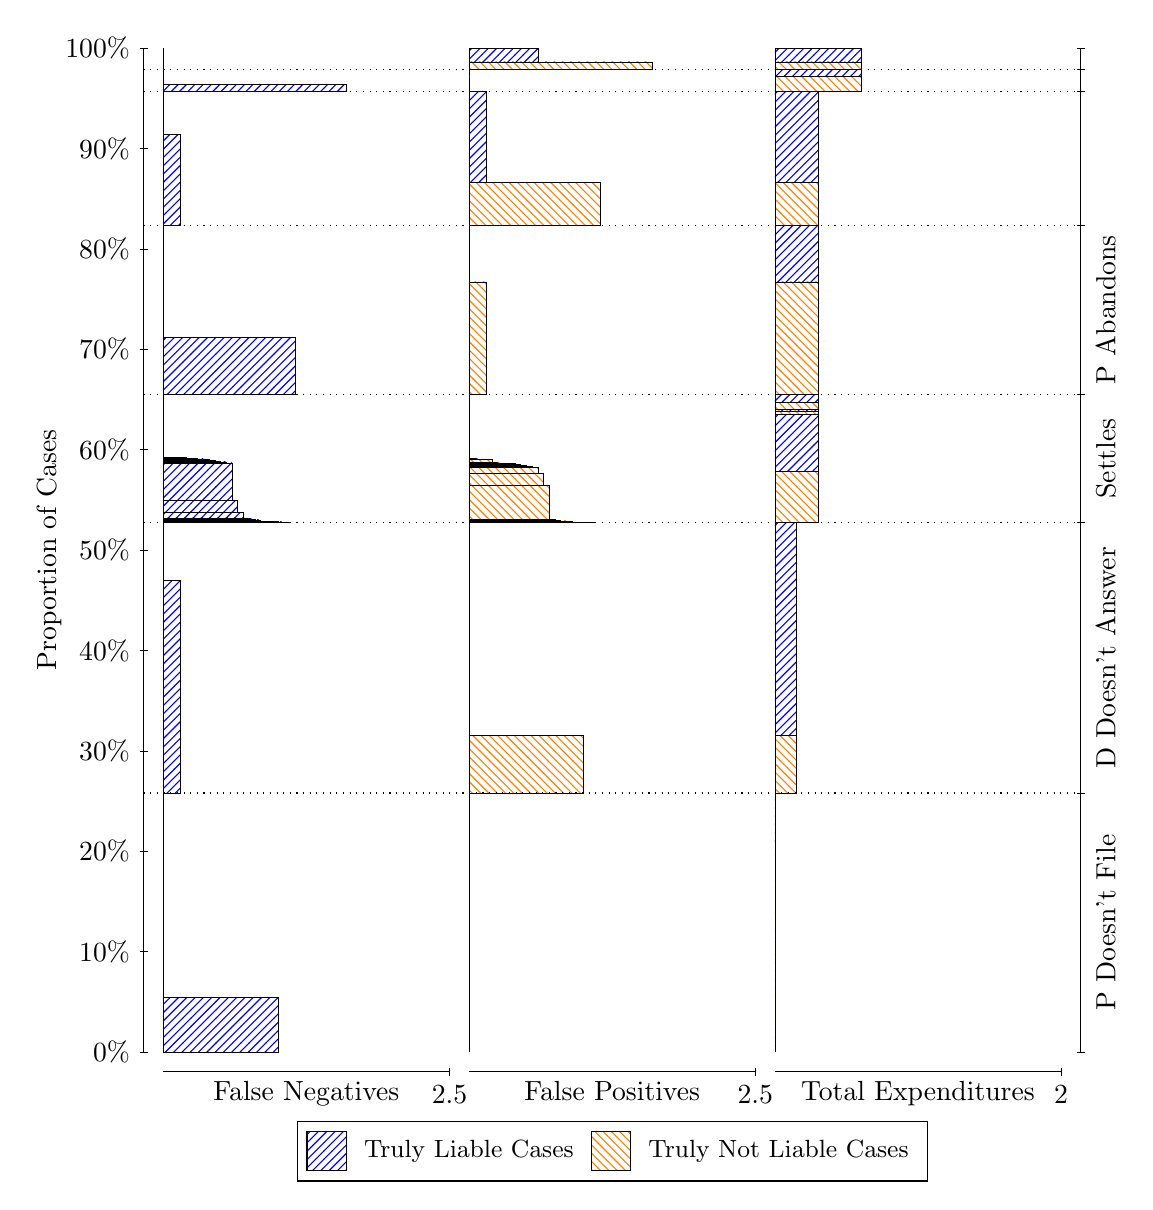
\begin{tikzpicture}
\draw[black, very thin] (1.5,1.75) -- (1.5,14.5);
\node[rotate=90, text=black, anchor=center] at (0.3, 8.125) {Proportion of Cases};
\draw[black, very thin] (1.45,1.75) -- (1.55,1.75);
\node[text=black, anchor=east] at (1.45, 1.75) {0\%};
\draw[black, very thin] (1.45,3.025) -- (1.55,3.025);
\node[text=black, anchor=east] at (1.45, 3.025) {10\%};
\draw[black, very thin] (1.45,4.3) -- (1.55,4.3);
\node[text=black, anchor=east] at (1.45, 4.3) {20\%};
\draw[black, very thin] (1.45,5.575) -- (1.55,5.575);
\node[text=black, anchor=east] at (1.45, 5.575) {30\%};
\draw[black, very thin] (1.45,6.85) -- (1.55,6.85);
\node[text=black, anchor=east] at (1.45, 6.85) {40\%};
\draw[black, very thin] (1.45,8.125) -- (1.55,8.125);
\node[text=black, anchor=east] at (1.45, 8.125) {50\%};
\draw[black, very thin] (1.45,9.4) -- (1.55,9.4);
\node[text=black, anchor=east] at (1.45, 9.4) {60\%};
\draw[black, very thin] (1.45,10.675) -- (1.55,10.675);
\node[text=black, anchor=east] at (1.45, 10.675) {70\%};
\draw[black, very thin] (1.45,11.95) -- (1.55,11.95);
\node[text=black, anchor=east] at (1.45, 11.95) {80\%};
\draw[black, very thin] (1.45,13.225) -- (1.55,13.225);
\node[text=black, anchor=east] at (1.45, 13.225) {90\%};
\draw[black, very thin] (1.45,14.5) -- (1.55,14.5);
\node[text=black, anchor=east] at (1.45, 14.5) {100\%};

\draw[black, very thin] (13.4,1.75) -- (13.4,14.5);
\draw[black, very thin] (13.35,1.75) -- (13.45,1.75);
\node[anchor=west] at (13.35, 1.75) {};
\draw[black, very thin] (13.35,5.0388) -- (13.45,5.0388);
\node[anchor=west] at (13.35, 5.0388) {};
\draw[black, very thin] (13.35,8.471) -- (13.45,8.471);
\node[anchor=west] at (13.35, 8.471) {};
\draw[black, very thin] (13.35,10.104) -- (13.45,10.104);
\node[anchor=west] at (13.35, 10.104) {};
\draw[black, very thin] (13.35,12.251) -- (13.45,12.251);
\node[anchor=west] at (13.35, 12.251) {};
\draw[black, very thin] (13.35,13.946) -- (13.45,13.946);
\node[anchor=west] at (13.35, 13.946) {};
\draw[black, very thin] (13.35,14.23) -- (13.45,14.23);
\node[anchor=west] at (13.35, 14.23) {};
\draw[black, very thin] (13.35,14.5) -- (13.45,14.5);
\node[anchor=west] at (13.35, 14.5) {};

\draw[black, very thin, pattern color=blue, pattern=north east lines] (1.75,1.75) rectangle (3.2033,2.448);
\draw[black, very thin, pattern color=orange, pattern=north west lines] (1.75,2.448) rectangle (1.75,5.0388);
\draw[black, very thin, pattern color=blue, pattern=north east lines] (1.75,5.0388) rectangle (1.968,7.7416);
\draw[black, very thin, pattern color=orange, pattern=north west lines] (1.75,7.7416) rectangle (1.75,8.471);
\draw[black, very thin, pattern color=blue, pattern=north east lines] (1.75,8.471) rectangle (3.3487,8.4801);
\draw[black, very thin, pattern color=blue, pattern=north east lines] (1.75,8.4801) rectangle (3.276,8.4831);
\draw[black, very thin, pattern color=blue, pattern=north east lines] (1.75,8.4831) rectangle (3.2033,8.4866);
\draw[black, very thin, pattern color=blue, pattern=north east lines] (1.75,8.4866) rectangle (3.1307,8.4878);
\draw[black, very thin, pattern color=blue, pattern=north east lines] (1.75,8.4878) rectangle (3.058,8.4933);
\draw[black, very thin, pattern color=blue, pattern=north east lines] (1.75,8.4933) rectangle (2.9853,8.5081);
\draw[black, very thin, pattern color=blue, pattern=north east lines] (1.75,8.5081) rectangle (2.9127,8.5118);
\draw[black, very thin, pattern color=blue, pattern=north east lines] (1.75,8.5118) rectangle (2.9127,8.5214);
\draw[black, very thin, pattern color=blue, pattern=north east lines] (1.75,8.5214) rectangle (2.84,8.5333);
\draw[black, very thin, pattern color=blue, pattern=north east lines] (1.75,8.5333) rectangle (2.7673,8.605);
\draw[black, very thin, pattern color=blue, pattern=north east lines] (1.75,8.605) rectangle (2.6947,8.7578);
\draw[black, very thin, pattern color=blue, pattern=north east lines] (1.75,8.7578) rectangle (2.622,8.7579);
\draw[black, very thin, pattern color=blue, pattern=north east lines] (1.75,8.7579) rectangle (2.622,9.2326);
\draw[black, very thin, pattern color=blue, pattern=north east lines] (1.75,9.2326) rectangle (2.5493,9.2352);
\draw[black, very thin, pattern color=blue, pattern=north east lines] (1.75,9.2352) rectangle (2.5493,9.243);
\draw[black, very thin, pattern color=blue, pattern=north east lines] (1.75,9.243) rectangle (2.4767,9.2431);
\draw[black, very thin, pattern color=blue, pattern=north east lines] (1.75,9.2431) rectangle (2.4767,9.2546);
\draw[black, very thin, pattern color=blue, pattern=north east lines] (1.75,9.2546) rectangle (2.404,9.2671);
\draw[black, very thin, pattern color=blue, pattern=north east lines] (1.75,9.2671) rectangle (2.3313,9.2778);
\draw[black, very thin, pattern color=blue, pattern=north east lines] (1.75,9.2778) rectangle (2.2587,9.281);
\draw[black, very thin, pattern color=blue, pattern=north east lines] (1.75,9.281) rectangle (2.186,9.2878);
\draw[black, very thin, pattern color=blue, pattern=north east lines] (1.75,9.2878) rectangle (2.1133,9.2918);
\draw[black, very thin, pattern color=blue, pattern=north east lines] (1.75,9.2918) rectangle (2.0407,9.3033);
\draw[black, very thin, pattern color=orange, pattern=north west lines] (1.75,9.3033) rectangle (1.75,10.104);
\draw[black, very thin, pattern color=blue, pattern=north east lines] (1.75,10.104) rectangle (3.4213,10.826);
\draw[black, very thin, pattern color=orange, pattern=north west lines] (1.75,10.826) rectangle (1.75,12.251);
\draw[black, very thin, pattern color=blue, pattern=north east lines] (1.75,12.251) rectangle (1.968,13.401);
\draw[black, very thin, pattern color=orange, pattern=north west lines] (1.75,13.401) rectangle (1.75,13.946);
\draw[black, very thin, pattern color=blue, pattern=north east lines] (1.75,13.946) rectangle (4.0753,14.04);
\draw[black, very thin, pattern color=orange, pattern=north west lines] (1.75,14.04) rectangle (1.75,14.23);
\draw[black, very thin, pattern color=orange, pattern=north west lines] (1.75,14.23) rectangle (1.75,14.323);
\draw[black, very thin, pattern color=blue, pattern=north east lines] (1.75,14.323) rectangle (1.75,14.5);
\draw[black, very thin, pattern color=orange, pattern=north west lines] (5.6333,1.75) rectangle (5.6333,4.3408);
\draw[black, very thin, pattern color=blue, pattern=north east lines] (5.6333,4.3408) rectangle (5.6333,5.0388);
\draw[black, very thin, pattern color=orange, pattern=north west lines] (5.6333,5.0388) rectangle (7.0867,5.7683);
\draw[black, very thin, pattern color=blue, pattern=north east lines] (5.6333,5.7683) rectangle (5.6333,8.471);
\draw[black, very thin, pattern color=orange, pattern=north west lines] (5.6333,8.471) rectangle (7.232,8.4736);
\draw[black, very thin, pattern color=orange, pattern=north west lines] (5.6333,8.4736) rectangle (7.1593,8.4749);
\draw[black, very thin, pattern color=orange, pattern=north west lines] (5.6333,8.4749) rectangle (7.0867,8.4772);
\draw[black, very thin, pattern color=orange, pattern=north west lines] (5.6333,8.4772) rectangle (7.014,8.4785);
\draw[black, very thin, pattern color=orange, pattern=north west lines] (5.6333,8.4785) rectangle (6.9413,8.4857);
\draw[black, very thin, pattern color=orange, pattern=north west lines] (5.6333,8.4857) rectangle (6.8687,8.495);
\draw[black, very thin, pattern color=orange, pattern=north west lines] (5.6333,8.495) rectangle (6.796,8.5038);
\draw[black, very thin, pattern color=orange, pattern=north west lines] (5.6333,8.5038) rectangle (6.796,8.5039);
\draw[black, very thin, pattern color=orange, pattern=north west lines] (5.6333,8.5039) rectangle (6.7233,8.5098);
\draw[black, very thin, pattern color=orange, pattern=north west lines] (5.6333,8.5098) rectangle (6.7233,8.5121);
\draw[black, very thin, pattern color=orange, pattern=north west lines] (5.6333,8.5121) rectangle (6.6507,8.9438);
\draw[black, very thin, pattern color=orange, pattern=north west lines] (5.6333,8.9438) rectangle (6.6507,8.944);
\draw[black, very thin, pattern color=orange, pattern=north west lines] (5.6333,8.944) rectangle (6.578,9.0973);
\draw[black, very thin, pattern color=orange, pattern=north west lines] (5.6333,9.0973) rectangle (6.5053,9.1715);
\draw[black, very thin, pattern color=orange, pattern=north west lines] (5.6333,9.1715) rectangle (6.4327,9.1832);
\draw[black, very thin, pattern color=orange, pattern=north west lines] (5.6333,9.1832) rectangle (6.36,9.1971);
\draw[black, very thin, pattern color=orange, pattern=north west lines] (5.6333,9.1971) rectangle (6.2873,9.209);
\draw[black, very thin, pattern color=orange, pattern=north west lines] (5.6333,9.209) rectangle (6.2873,9.2137);
\draw[black, very thin, pattern color=orange, pattern=north west lines] (5.6333,9.2137) rectangle (6.2147,9.2208);
\draw[black, very thin, pattern color=orange, pattern=north west lines] (5.6333,9.2208) rectangle (6.142,9.2231);
\draw[black, very thin, pattern color=orange, pattern=north west lines] (5.6333,9.2231) rectangle (6.0693,9.2308);
\draw[black, very thin, pattern color=orange, pattern=north west lines] (5.6333,9.2308) rectangle (5.9967,9.2381);
\draw[black, very thin, pattern color=orange, pattern=north west lines] (5.6333,9.2381) rectangle (5.924,9.2719);
\draw[black, very thin, pattern color=blue, pattern=north east lines] (5.6333,9.2719) rectangle (5.7787,9.2834);
\draw[black, very thin, pattern color=blue, pattern=north east lines] (5.6333,9.2834) rectangle (5.706,9.2874);
\draw[black, very thin, pattern color=blue, pattern=north east lines] (5.6333,9.2874) rectangle (5.6333,10.104);
\draw[black, very thin, pattern color=orange, pattern=north west lines] (5.6333,10.104) rectangle (5.8513,11.53);
\draw[black, very thin, pattern color=blue, pattern=north east lines] (5.6333,11.53) rectangle (5.6333,12.251);
\draw[black, very thin, pattern color=orange, pattern=north west lines] (5.6333,12.251) rectangle (7.3047,12.796);
\draw[black, very thin, pattern color=blue, pattern=north east lines] (5.6333,12.796) rectangle (5.8513,13.946);
\draw[black, very thin, pattern color=orange, pattern=north west lines] (5.6333,13.946) rectangle (5.6333,14.136);
\draw[black, very thin, pattern color=blue, pattern=north east lines] (5.6333,14.136) rectangle (5.6333,14.23);
\draw[black, very thin, pattern color=orange, pattern=north west lines] (5.6333,14.23) rectangle (7.9587,14.323);
\draw[black, very thin, pattern color=blue, pattern=north east lines] (5.6333,14.323) rectangle (6.5053,14.5);
\draw[black, very thin, pattern color=orange, pattern=north west lines] (9.5167,1.75) rectangle (9.5167,4.3408);
\draw[black, very thin, pattern color=blue, pattern=north east lines] (9.5167,4.3408) rectangle (9.5167,5.0388);
\draw[black, very thin, pattern color=orange, pattern=north west lines] (9.5167,5.0388) rectangle (9.7892,5.7683);
\draw[black, very thin, pattern color=blue, pattern=north east lines] (9.5167,5.7683) rectangle (9.7892,8.471);
\draw[black, very thin, pattern color=orange, pattern=north west lines] (9.5167,8.471) rectangle (10.062,9.128);
\draw[black, very thin, pattern color=blue, pattern=north east lines] (9.5167,9.128) rectangle (10.062,9.8425);
\draw[black, very thin, pattern color=orange, pattern=north west lines] (9.5167,9.8425) rectangle (10.062,9.8921);
\draw[black, very thin, pattern color=blue, pattern=north east lines] (9.5167,9.8921) rectangle (10.062,9.9081);
\draw[black, very thin, pattern color=orange, pattern=north west lines] (9.5167,9.9081) rectangle (10.062,10.002);
\draw[black, very thin, pattern color=blue, pattern=north east lines] (9.5167,10.002) rectangle (10.062,10.104);
\draw[black, very thin, pattern color=orange, pattern=north west lines] (9.5167,10.104) rectangle (10.062,11.53);
\draw[black, very thin, pattern color=blue, pattern=north east lines] (9.5167,11.53) rectangle (10.062,12.251);
\draw[black, very thin, pattern color=orange, pattern=north west lines] (9.5167,12.251) rectangle (10.062,12.796);
\draw[black, very thin, pattern color=blue, pattern=north east lines] (9.5167,12.796) rectangle (10.062,13.946);
\draw[black, very thin, pattern color=orange, pattern=north west lines] (9.5167,13.946) rectangle (10.607,14.136);
\draw[black, very thin, pattern color=blue, pattern=north east lines] (9.5167,14.136) rectangle (10.607,14.23);
\draw[black, very thin, pattern color=orange, pattern=north west lines] (9.5167,14.23) rectangle (10.607,14.323);
\draw[black, very thin, pattern color=blue, pattern=north east lines] (9.5167,14.323) rectangle (10.607,14.5);
\draw[black, dotted] (1.5,5.0388) -- (13.4,5.0388);
\draw[black, dotted] (1.5,8.471) -- (13.4,8.471);
\draw[black, dotted] (1.5,10.104) -- (13.4,10.104);
\draw[black, dotted] (1.5,12.251) -- (13.4,12.251);
\draw[black, dotted] (1.5,13.946) -- (13.4,13.946);
\draw[black, dotted] (1.5,14.23) -- (13.4,14.23);
\draw[black, very thin] (1.75,1.5) -- (5.3833,1.5);
\node[text=black, anchor=north] at (3.5667, 1.5) {False Negatives};
\draw[black, very thin] (5.3833,1.45) -- (5.3833,1.55);
\node[text=black, anchor=north] at (5.3833, 1.45) {2.5};

\draw[black, very thin] (5.6333,1.5) -- (9.2667,1.5);
\node[text=black, anchor=north] at (7.45, 1.5) {False Positives};
\draw[black, very thin] (9.2667,1.45) -- (9.2667,1.55);
\node[text=black, anchor=north] at (9.2667, 1.45) {2.5};

\draw[black, very thin] (9.5167,1.5) -- (13.15,1.5);
\node[text=black, anchor=north] at (11.333, 1.5) {Total Expenditures};
\draw[black, very thin] (13.15,1.45) -- (13.15,1.55);
\node[text=black, anchor=north] at (13.15, 1.45) {2};

\node[text=black, centered, rotate=90] at (13.72, 3.3944) {\contour{white}{P Doesn't File}};
\node[text=black, centered, rotate=90] at (13.72, 6.7549) {\contour{white}{D Doesn't Answer}};
\node[text=black, centered, rotate=90] at (13.72, 9.2876) {\contour{white}{Settles}};
\node[text=black, centered, rotate=90] at (13.72, 11.178) {\contour{white}{P Abandons}};




\draw (7.449999999999999,1.5) node[draw=none] (baseCoordinate) {};
\begin{scope}[align=center]
        \matrix[scale=0.5, draw=black, below=0.5cm of baseCoordinate, nodes={draw}, column sep=0.1cm]{
            \node[rectangle, draw, minimum width=0.5cm, minimum height=0.5cm, pattern color=blue, pattern=north east lines] {}; &
            \node[draw=none, font=\small, text=black] (B) {Truly Liable Cases}; &
            \node[rectangle, draw, minimum width=0.5cm, minimum height=0.5cm, pattern color=orange, pattern=north west lines] {}; &
            \node[draw=none, font=\small, text=black] (B) {Truly Not Liable Cases}; \\
            };
\end{scope}

\end{tikzpicture}
\end{document}